Одной из наиболее проработанных научных психологических теорий интеллектуального развития 
является теория когнитивного развития, разработанная Жаном Пиаже \cite{piaget1952origins}.
Когнитивное развитие происходит в форме стадий, соответствующих развитию интеллектуальных
способностей. Таковыми являются все виды мыслительных процессов, таких как восприятие,
память, формирование понятий, решение задач, воображение и логика.

Этапы развития детской психики по Жану Пиаже:
\begin{enumerate}
    \item Этап сенсомоторного интеллекта соответствует возрасту от рождения до 2 лет. 
    Он характеризуется развитием моторной памяти и овладением основными чувствами: зрениям, слухом и балансом.
    \item Этап дооперационального представления происходит с двух до семи лет. На этой стадии дети еще не могут
    применять конкретные когнитивные операции, не могут использовать математический счет и язык для практических целей.
    Объекты мира представляются идеальными согласно желаниям ребенка. Тем не менее текущих навыков достаточно для самостоятельного ухода
    за собой и одеждой, совместной социальной деятельности и детского творчества.
    \item Период конкретных операций от семи до одиннадцати лет. Ребенок способен на дедуктивное и индуктивное мышление.
    \item Конкретное и абстрактное логическое мышление соответствует ментальному развитию взрослого человека. Подросток понимает
    литературный язык, способен на логическое оформление творческой мысли.
\end{enumerate}

Пиаже обосновывает свою теорию этичными экспериментами, легко доступными к воспроизведению педагогами.
Инструментами научного эксперимента являются зеркала, куклы, пластилин и игры для детей. Изучаются реакция ребенка
на сокрытие куклы за тканью, понимание сохранения материи на примере лепки и осознание своей личности при наблюдении
за отражением в зеркале.

\begin{figure}[h]
    \centering
    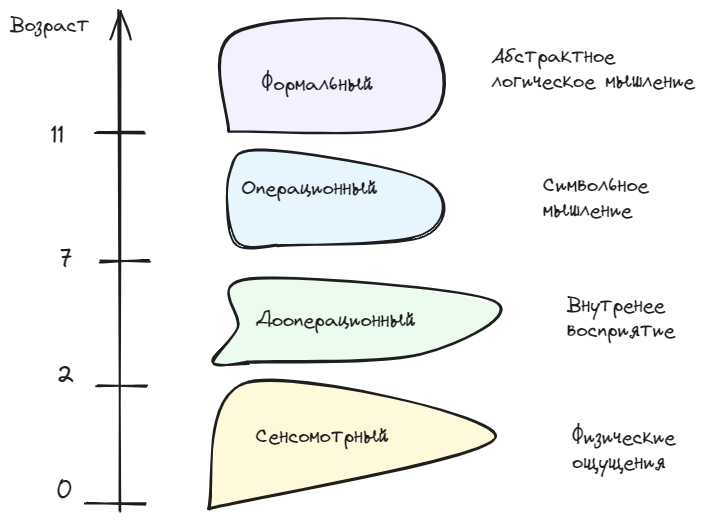
\includegraphics[width=0.5\textwidth]{assets/pedagogic/psy/piage.excalidraw.png}
    \caption{Этапы развития детской психики по Жану Пиаже \cite{piaget1952origins}}
    \label{piage}
\end{figure}

Лев Семёнович Выготский оспаривает этот подход, приводя в пример детей, которые в ходе занятий со взрослыми продемонстрировали
высокий уровень освоения шахмат \ref{proximal_growth}. Выполненные Выготским
эксперименты стали основой направления культурно-исторической психологии, признанной в мировом профессиональном сообществе.
Согласно Выготскомуб образование имеет социальный и целенаправленный характер и связанно с развитием
\textit{высших психических функции} --- сложных самоорганизующихся процессов в деятельности человека, 
опосредованных знаками по своему строению и произвольных по способу своего осуществления. В качестве таких навыков Выготский
определяет мышление, речь, произвольное внимание, волю, воображение и др.

\textit{Определение:} \textbf{Зона ближайшего развития} --- расхождение между уровнем актуального психического развития ребёнка
 и уровнем его потенциального развития, достигаемого при решении задач в сотрудничестве со взрослым или сверстниками. 

\begin{figure}[h]
    \centering
    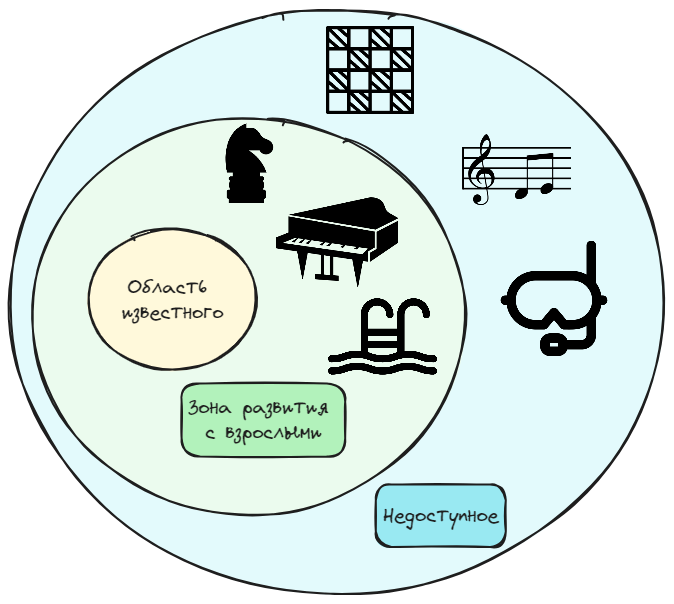
\includegraphics[width=0.35\textwidth]{assets/pedagogic/psy/proximal_growth.excalidraw.png}
    \caption{Иллюстрация границ зон развития согласно Л.С. Выготскому}
    \label{proximal_growth}
\end{figure}

Согласно Выготскому ключевым для образовании является процесс рефлексии учащегося.
Такой процесс включает в себя осознанный анализ своего учебного опыта, рассмотрение своих мыслей, чувств и действий в контексте обучения. 
Механизмом рефлексии является \textit{интериоризация}. Процесс заключается в переходе внешней речи во внутренний способ мышления.
Отметим, что процесс возможен когда ребёнок уже способен планировать свою деятельность. 
 
\begin{figure}[h]
    \centering
    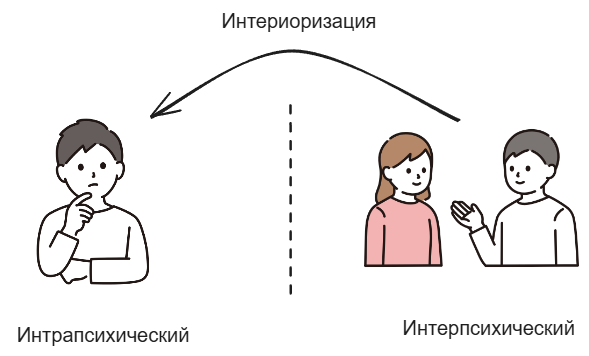
\includegraphics[width=0.5\textwidth]{assets/pedagogic/psy/reflection.excalidraw.png}
    \caption{Рефлексия по Выготскому \cite{выготский2014мышление}}
    \label{reflection}
\end{figure}
 
 Рефлексия способствует развитию метакогнитивных навыков:
  \begin{itemize}
     \item оценки своей деятельности и планирования;
     \item осознания ценности знания и социума;
     \item ведения высшей когнитивной деятельности по организации социальной деятельности.
 \end{itemize}
Такие навыки позволяют справляться с практическими заданиями, обучать и осваивать неизвестные области знания,
выявлять пробелы в знаниях и развивать критическое мышление.

\textit{Определение:} \textbf{Поток} (от \textit{лат.} influunt) по Чиксентмихайи --- это психическое состояние, характеризующееся полной вовлеченностью и концентрацией
на текущей деятельности, сопровождающееся ощущением контроля, потерей чувства времени и высокой внутренней мотивацией.

Теория потока активно используется в играх \cite{chen2007flow} и программах непрерывного обучения \cite{jarvis2009routledge} для
задания оптимальной сложности образовательной программы.

\begin{figure}[h]
    \centering
    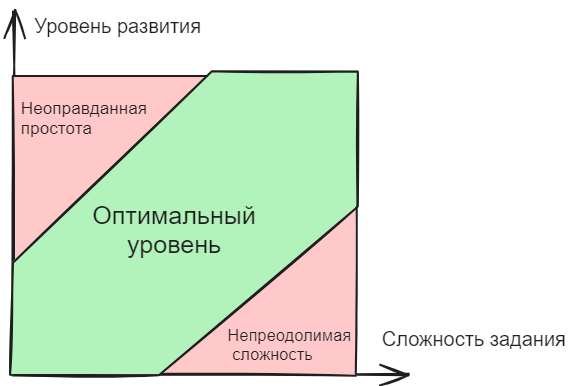
\includegraphics[width=0.5\textwidth]{assets/pedagogic/psy/flow.excalidraw.png}
    \caption{Модель оптимальной сложности согласно Михаю Чиксентмихайи}
    \label{flow_model}
\end{figure}

Характеристиками потока согласно \cite{csikszentmihalyi2005flow} являются:
 \begin{itemize}
    \item Ясные цели и обратная связь. Деятельность имеет чёткие цели и предоставляет немедленную обратную связь.
    \item Баланс между сложностью задачи и навыками. Задача должна быть достаточно сложной, чтобы представлять собой вызов, 
    но при этом соответствовать уровню навыков человека, чтобы не вызывать скуки и тревоги.
    \item Слияние действия и сознания. Человек настолько поглощён деятельностью, что все его действия становятся почти автоматическими и интуитивными.
    \item Потеря самосознания. В потоке человек забывает о себе, своих заботах и тревогах, полностью сосредоточившись на задаче.
    \item Искажение восприятия времени. Время может казаться летящим быстро или, наоборот, замедляться; часы могут пройти как минуты
\end{itemize}


\textit{Определение:} \textbf{Гипотеза о врожденных знаниях}(от \textit{англ.} Innateness hypothesis) --- теория в лингвистике и когнитивной науке,
 которая утверждает, что способность к языку является врождённой характеристикой человеческого мозга. 

Гипотеза постулирует наличие:
\begin{itemize}
    \item врождённого языкового аппарата, способствующего естественному освоению языка;
    \item универсальной грамматики, состоящей из набора грамматических принципов и структур, присутствующих во всех языках и врождённых для каждого человека;
    \item основных аспектов языковой способности, являющихся врождёнными и не зависящими от окружающей среды.
\end{itemize}

Гипотеза имеет статистические подтверждения, описанные в работах Хоам Номски, использовавшего статистический аппарат синтаксических деревьев 
для анализа массивного корпуса естественного языка \cite{everaert2015structures}\cite{montague1970universal}.




